\chapter{Požadavky a architektura prostředí pro NVF a VFN}

V předešlé kapitole byla vysvětlena základní problematika, která souvisí s virtualizací síťových funkcí, cloud computingem a softwarově definovanými sítěmi. Zároveň byla popsána referenční architektura frameworku pro virtualizaci síťových funkcí. Tato kapitola bude již věnována konkrétnímu příkladu využití virtuálních síťových funkcí v cloudovém prostředí. Nejprve zde popsána navržená architektura pro privátní cloudovou platformu využívající virtualizaci síťových funkcí, kterou mohou využívat všichni její uživatelé. Pro tuto cloudovou platformu a pro její uživatele byli navrženy dva příklady virtuálních síťových funkcí. U obou příkladů jsou uvedeny scénáře a způsob jakým jsou navrženy.

\section{Požadavky na NFV Infrastrukturu}

//Open Source technologie 

//Možnost automatického vytváření ifrastruktury

//Podporara různých řešení pro SDN

//Vybral jsem si OpenStack protože ...

\section{Požadavky na VNF}

Vybral jsem si PFSense a Fortigate ...

Vybral jsem si HAproxy a AVI networks ...

\section{Výsledná architektura použitého frameworku}

Architektura navrženého řešení byla implementována pomocí cloudové platformy OpenStack a SDN řešení OpenContrail. Obrázku č. \ref{fig:VNF_overview} znázorňuje tyto technologie v souvislosti s referenční architekturou popsanou v kapitole \ref{sub:architektura}. Je nutné říci, že obě technologie nezapadají přímo do jedné z částí referenční architektury. Naopak v některých případech se překrývají nebo se v ní doplňují.

\begin{figure}[h]
\begin{centering}
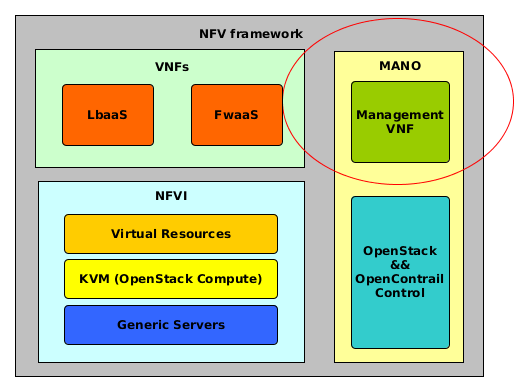
\includegraphics[scale=0.51]{images/VNF_overview}
\par\end{centering}
\caption{Architektura NFV řešení\label{fig:VNF_overview}}
\end{figure}

OpenStack byl zvolen, protože se jedná o největší open-source cloudovou platformu na světě. OpenStack tvoří část správy infrastruktury. Hardwarová vrstva infrastruktury se může skládat z libovolných serverů, na kterých je nainstalován KVM hypervizor. Tento hypervizor tvoří virtuální vrsvu a byl vybrán, protože je nejčastěji používán společně s OpenStackem. Avšak v případě potřeby by zde mohl být použit i jiný hypervizor, pokud bude zachována kompatibilita vůči OpenStacku.

OpenStack spravuje převážně zdroje týkající se výpočeního výkonu (Compute) a uložiště (Storage). Tyto zdroje následně přiděluje dle potřeby virtuálním instancím nebo v našem případě instancím, které slouží jako VNF. Bylo však nutné zvolit řešení, které se bude starat o síťování.

Speciálně pro vyřešení síťování v této infrastruktuře je součástí řešení OpenContrail. Díky tomu je možné vytvářet overlay sítě pomocí VXLAN či MPLS over GRE, kterými jsou dynamicky propojovány jednotlivé VM a VNF. 

Jednotlivá VNF mohou být v OpenContrailu vytvořena pomocí tzv. Servisních Instance a Servisní Templatů. Ty budou v této práci použity pro vytvoření VNF sloužící jako firewally a budou podrobně popsány v kapitole věnující se vytváření této služby.

Další součástí, která musela být v architektuře navrhnuta, je způsob řízení a správy jednotlivých VNF. Zde se muselo jednat o řešení, jakým automaticky vytvořit a popřípadě i smazat všechny potřebné části potřebné pro VNF. Pro tuto část byl zvolen Heat. Heat je část OpenStacku, která slouží pro automatickou orchestraci. Ten bude v tomto návrhu zastávat roli VFN managera, pomocí kterého budou jednotlivé VNF spravovány. Avšak dalo by se říci, že do této role spadá i OpenContrail, protože právě on umožnuje také spravovat jednostlivá VNF za běhu.  

Heat je hlavní projekt v OpenStacku pro orchestraci. Umožňuje uživatelům popsat nasazení komplexních cloudových aplikací v jednom textovém souboru, který se nazývá Heat template. Tyto soubory se dají předat heat enginu, který podle nich dokáže automaticky vytvořit požadované zdroje v OpenStacku i v OpenContrailu. 


Z toho návrhu je patrné, že zde není implementovaný NFV orchestrator. Je to z důvodu toho, že pro účely řešení virtuálních síťových funkcí na cloudové platformě OpenStack s OpenContrailem, která je navržena v této práci, není tato část potřeba.



